\section{Gruppen-�berblick}Auf dieser Seite sehen Sie Ihre Client-Gruppen und die Anzahl der jeweils darin enthaltenen Clients. Durch einen Klick auf den Gruppennamen sehen Sie die Detail-Seite der jeweiligen Gruppe.\\
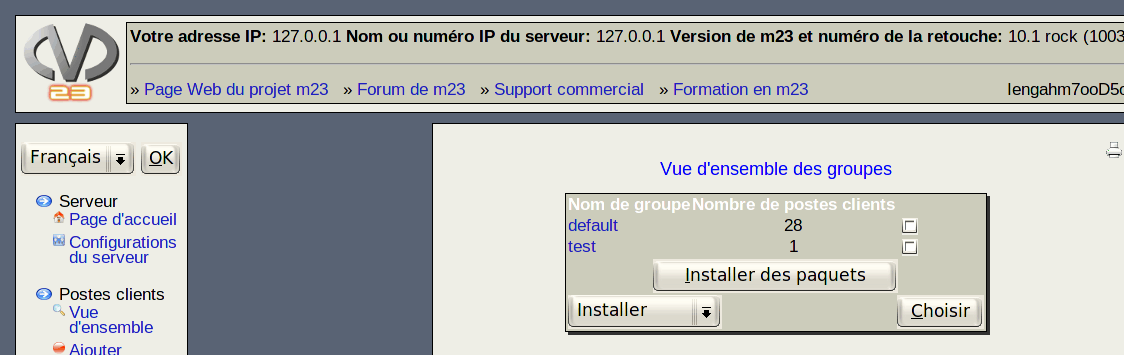
\includegraphics[scale=0.4]{/mdk/doc/manual/screenshots/de/groups_overview.png} \\
\subsection{Auftr�ge an eine Gruppe �bergeben}
Sie k�nnen Auftr�ge an die Clients einer oder mehrerer Gruppen �bergeben und somit die Administration bei der Installation, Deinstallation oder beim Update stark vereinfachen.\\
\subsection{Gehen Sie dazu wie folgt vor:}
\begin{itemize}
\item W�hlen Sie die gew�nschte Aktion aus der Liste.\\
\item Klicken Sie auf \textit{"W�hlen"}, worauf die Beschriftung des Aktions-Buttons die gew�hlte Aktion anzeigen sollte.\\
\item W�hlen Sie die Gruppe(n) aus.\\
\item Klicken Sie schlie�lich 2x auf den Aktions-Button.\\
\end{itemize}
